\documentclass[24pt]{beamer}
\usepackage[orientation=portrait, size=custom, width=84.1, height=59.4,scale=1.2]{beamerposter}
\usepackage[absolute,overlay]{textpos}
\usepackage{bookmark} %pdflatex says to use this to avoid errors...
\usepackage{graphicx} %for including images
\graphicspath{{figs/}} %location of images
\usepackage{wrapfig} %wrap text around the images
\usepackage{listingsutf8}    %package for code environment; use this instead of verbatim to get automatic line break; use this instead of listings to get (•)
\usepackage{amsmath}
\usepackage{gensymb}
\usepackage[export]{adjustbox}
\usepackage[skins,theorems]{tcolorbox}
\usepackage{tikz}
\newcommand*\circled[1]{\tikz[baseline=(char.base)]{
            \node[shape=circle,draw,inner sep=2pt] (char) {#1};}}
\usepackage{array}
\usepackage{booktabs,adjustbox}
\usepackage{subcaption}
\usepackage{pgfplots}
\usepackage{pgf-pie}  % for pie charts
%plot options
\pgfplotsset{width=7cm,compat=1.8}
\PassOptionsToPackage{gray}{xcolor}
\usepackage{cite}
\usepackage{fancyvrb}
%\usepackage{minted}

\usetikzlibrary{shapes,shapes.geometric,arrows,fit,calc,positioning,automata,}

\usepackage{wrapfig}

%\mode<presentation>
%this doesn't seem to make any difference; leave for now for trying out
\usetheme{Berlin}
\definecolor{MacBlue}{rgb}{0.10196,0.22353,0.53725}
\definecolor{MacMaroon} {rgb}{0.47843, 0, 0.23137}
\definecolor{MacMaroon2} {rgb}{0.47451, 0, 0}
\definecolor{MacGray}{rgb}{0.50196,0.49804,0.51765}
\definecolor{MacMaroon3}{rgb}{00.47,0.2,0.31}
\definecolor{MacGold}{rgb}{1, 0.75,0.35}

\definecolor{INTERpos}{RGB}{188, 236, 172} % Soft sage green
\definecolor{ELMpos}{RGB}{178, 255, 102} % Light lime green
\definecolor{ONL}{RGB}{178, 229, 102} % Pastel olive
\definecolor{IRL}{RGB}{229, 229, 102} % Pastel yellow
\definecolor{ANX}{RGB}{255, 204, 102} % Light orange
\definecolor{CODE}{RGB}{255, 178, 102} % Soft orange
\definecolor{INTERneg}{RGB}{255, 102, 102} % Soft red
\definecolor{FOCUS}{RGB}{0, 119, 179} % Cornflower blue
\definecolor{CAPT}{RGB}{255, 153, 255} % Light purple
\definecolor{GPT}{RGB}{204, 153, 255} % Lavender
\definecolor{DEEPEN}{RGB}{85, 0, 204} % Rich indigo
\definecolor{QAmov}{RGB}{153, 153, 255} % Soft blue
\definecolor{NOISE}{RGB}{102, 178, 255} % Sky blue
\definecolor{LENinc}{RGB}{102, 204, 255} % Light cyan
\definecolor{LENdec}{RGB}{102, 229, 204} % Aqua green
\definecolor{ROUNDpos}{RGB}{153, 204, 0} % Muted lime
\definecolor{TIME}{RGB}{197, 204, 102} % Muted olive
\definecolor{DEBAT}{RGB}{204, 204, 102} % Muted yellow
\definecolor{BREAK}{RGB}{204, 179, 102} % Muted orange
\definecolor{ROUNDneg}{RGB}{150, 54, 86} % Burgundy
\definecolor{ELMneg}{RGB}{229, 102, 102} % Soft red
\definecolor{RUBR}{RGB}{204, 102, 153} % Soft raspberry
\definecolor{OUTCOME}{RGB}{204, 102, 204} % Muted purple
\definecolor{PROCESS}{RGB}{153, 102, 204} % Soft violet
\definecolor{PROF}{RGB}{102, 102, 204} % Periwinkle
\definecolor{LIVE}{RGB}{102, 153, 204} % Denim blue
\definecolor{ACCOUNT}{RGB}{102, 178, 204} % Soft teal
\definecolor{PACE}{RGB}{102, 204, 204} % Soft turquoise
\definecolor{ANON}{RGB}{102, 204, 178} % Mint green
\definecolor{SIZE}{RGB}{210, 210, 162} % Beige
\definecolor{PERS}{RGB}{255, 255, 178} % Pale lemon
\definecolor{PREREQ}{RGB}{255, 204, 178} % Light peach
\definecolor{RESOURCE}{RGB}{255, 204, 255} % Pink lavender
\definecolor{ENGL}{RGB}{178, 178, 255} % Very soft blue
\definecolor{TIMEMGMT}{RGB}{204, 153, 201} % Muted dusky rose
\definecolor{QAinc}{RGB}{224, 224, 255} % Softest blue
\definecolor{CONCISE}{RGB}{224, 255, 255} % Pale cyan
\definecolor{RELEVANT}{RGB}{224, 224, 224} % Very light grey
\definecolor{COMMON}{RGB}{178, 178, 178} % Light grey

% Code from https://stackoverflow.com/questions/78627262/tikz-picture-pie-chart-exclude-labels-for-categories-with-0 to fix the 0-label issue
\makeatletter
% args:
% #1: begin angle
% #2: end angle
% #3: number
% #4: label
% #5: explode
% #6: fill color
% #7: radius
% #8: center
\def\pgfpie@slice#1#2#3#4#5#6#7#8{%
  \pgfmathparse{0.5*(#1)+0.5*(#2)}
  \let\pgfpie@midangle\pgfmathresult

  \path (#8) -- ++({\pgfpie@midangle}:{#5}) coordinate (pgfpie@O);

  \pgfmathparse{(#7)+(#5)}
  \let\pgfpie@radius\pgfmathresult
  
  % slice
  \draw[line join=round,fill={#6},\pgfpie@style] (pgfpie@O) -- ++({#1}:{#7}) arc ({#1}:{#2}:{#7}) -- cycle;

  \pgfpie@ifchangedirection{%
    \pgfmathparse{min(((#1)-(#2)-10)/110*(-0.3),0)}
  }{%
    \pgfmathparse{min(((#2)-(#1)-10)/110*(-0.3),0)}
  }%
  \let\pgfpie@minresult\pgfmathresult

  \pgfmathparse{(max(\pgfpie@minresult,-0.5) + 0.8)*(#7)}
  \let\pgfpie@innerpos\pgfmathresult

  \pgfpie@ifx\pgfpie@text\pgfpie@text@inside{%
    % label and number together
    \path (pgfpie@O) -- ++({\pgfpie@midangle}:{\pgfpie@innerpos}) node[align=center]
    {\pgfpie@scalefont{#3}\pgfpie@labeltext{#4}\\\pgfpie@numbertext{#3}};
  }{%
    % label
    \pgfpie@ifhidelabel{}{%
      \pgfpie@iflegend{}{%
        \path (pgfpie@O) -- ++ ({\pgfpie@midangle}:{\pgfpie@radius})
        node[inner sep=0, \pgfpie@text={\pgfpie@midangle:#4}]{};
      }%
    }%

    \pgfmathparse{max((#1)-(#2),(#2)-(#1))}
    \let\pgfpie@sliceangle\pgfmathresult

    \pgfmathparse{max(1, min(20-\pgfpie@sliceangle,1.5))}
    \let\pgfpie@multiplier\pgfmathresult

    % number
    \ifnum#3>0
      % \ifnum{\pgfpie@pieangle}<0.785
        % Place the label outside the pie chart if #3 is 1
        \path (pgfpie@O) -- ++({\pgfpie@midangle}:{\pgfpie@multiplier*\pgfpie@innerpos}) node
        {\pgfpie@scalefont{#3}\pgfpie@numbertext{#3}};
      % \else
      %   % Place the label inside the pie chart for other values of #3
      %   \path (pgfpie@O) -- ++({\pgfpie@midangle}:{\pgfpie@innerpos}) node
      %   {\footnotesize\pgfpie@scalefont{#3}\pgfpie@numbertext{#3}};
    \fi
  }%
}

\def\pgfpie@text@blank{blank}

\def\pgfpie@legend#1{%
  \coordinate[xshift=1.2cm,
  yshift={(\the\pgfpie@sliceLength*0.5+3.5)*0.5cm}] (pgfpie@legendpos) at
  (current bounding box.east);

  \scope[node distance=1cm]
    \foreach \pgfpie@p/\pgfpie@t [count=\pgfpie@i from 0] in {#1}
    {
      \pgfpie@findColor{\pgfpie@i}
      \node[draw, fill={\pgfpie@thecolor}, \pgfpie@style, below of={pgfpie@legendpos}, label={0:{\pgfpie@t}}] (pgfpie@legendpos) {};
    }
  \endscope
}
\makeatother

\usecolortheme[named=MacMaroon2]{structure}
\setbeamertemplate{caption}[numbered]
\setbeamertemplate{navigation symbols}{}

\title{A Functional Event-Driven Framework}
\subtitle{}
\author[Schankula, Smith \& Anand]{Christopher William Schankula, Spencer Smith, \\Christopher K. Anand$^\dagger$ \newline \small \{schankuc, smiths, anandc\}@mcmaster.ca}
\institute[McMaster University]{$^\dagger$Department of Computing and Software, McMaster University \quad \texttt{https://stablfoundation.org}, \texttt{http://outreach.mcmaster.ca}}
\date{November, 2024}

\setbeamerfont{title}{size=\huge}

\makeatletter
\setbeamertemplate{title page}{
  \vbox{}
  \vfill
  \begingroup
    \centering
    \begin{beamercolorbox}[sep=8pt,center]{title}
      \usebeamerfont{title}\inserttitle\par%
      \ifx\insertsubtitle\@empty%
      \else%
        \vskip0.25em%
        {\usebeamerfont{subtitle}\usebeamercolor[fg]{subtitle}\insertsubtitle\par}%
      \fi%     
    \end{beamercolorbox}%
    \vskip0.5em\par % reduce spacing between title and author
    \begin{beamercolorbox}[sep=8pt,center]{author}
      \usebeamerfont{author}\insertauthor
    \end{beamercolorbox}
    \begin{beamercolorbox}[sep=8pt,center]{institute}
      \usebeamerfont{institute}\insertinstitute
    \end{beamercolorbox}
    % ------------------------
    \begin{beamercolorbox}[sep=8pt,center]{date}
      \usebeamerfont{date}\insertdate
    \end{beamercolorbox}
    {\usebeamercolor[fg]{titlegraphic}\inserttitlegraphic\par}
  \endgroup
  \vfill
}
\makeatother

\begin{document}
%compile with pdflatex

%there is only one frame, because there is only one page; yeah, it's a poster
%textblock and block seem to work nicely to organize layout
\begin{frame}[fragile]

\begin{textblock}{2}(0.5,0.75)

\includegraphics[width=14cm]{eng_logo.png} % We can use CAS logo as well?
\end{textblock}

\begin{textblock}{2}(12.7,0.75)

\includegraphics[width=14cm, trim= 0 0 1cm 0, clip]{STaBLLogoWS.png}
\end{textblock}

\begin{textblock}{9}(3.5,0.5)
\titlepage
\end{textblock}

\begin{textblock}{7.25}(0.5,2.9)

%this needs help
\begin{block}{\fontsize{37}{20}\selectfont Background}
Elm is a \textbf{strongly-typed, pure functional programming language}. It is used to create type-safe 
front-end web applications, but concurrent applications require writing separate 
server code and client-server communication code. This project explores
\textbf{serverless development} in Elm, and its effect on the engagement of new 
programmers.
% The Elm Architecture (also known as model-view-update or MVU) consists of a model, 
% describing the data in the application as well as a pure update function, which
% returns a new model (state) and a pure view function which 
\vspace{5mm}
\end{block}

\begin{block}{\fontsize{37}{20}\selectfont Novel Architecture}
\begin{itemize}
    \item Builds on Elm's MVU, with a local (private) and global (shared) model and update
\end{itemize}
\begin{figure}
%\includegraphics[height = 15cm, trim= 24.5cm 0 0 4cm, clip]{TEASync.png}
\caption{A two-client dataflow diagram of the Local-Global Model-View-Update Architecture. Each client has its own local model (top and bottom band), and all clients share a global model (middle band).}
\label{Fig:TEA}
\end{figure}
\vspace{-6mm}
\end{block}

\begin{block}{\fontsize{37}{20}\selectfont Conclusions \& Future Work}
Leveraging the strictly-typed nature of Elm and its MVU architecture, we were able
to create a \textbf{simplified multi-user framework}, with no application-specific 
server-side code. First-year students were able to create \textbf{complex multiplayer
games} and surveyed students reported a high level of enjoyment. Ongoing work includes 
formalizing visual models for creating TEASync 
applications.
\end{block}


\begin{block}{\fontsize{37}{20}\selectfont Acknowledgments}
We thank NSERC for CGS-M funding and the Government of Ontario for OGS funding. 
Thanks to CS 1XD3 group 42 (*) for allowing inclusion of
their apps as an example. Special thanks to Denise Geiskkovitch for helping with the 
usability and engagement study.
\end{block}

\begin{figure}[htbp]
\centering

\includegraphics[height=3.2cm,trim={0 0 28.5cm 0},clip]{nserc-logo.jpg}
\hspace{0.5cm}

\includegraphics[height=3.2cm,trim={16.5cm 0 0 0},clip]{ontario@2x-print.png}
\hspace{0.5cm}
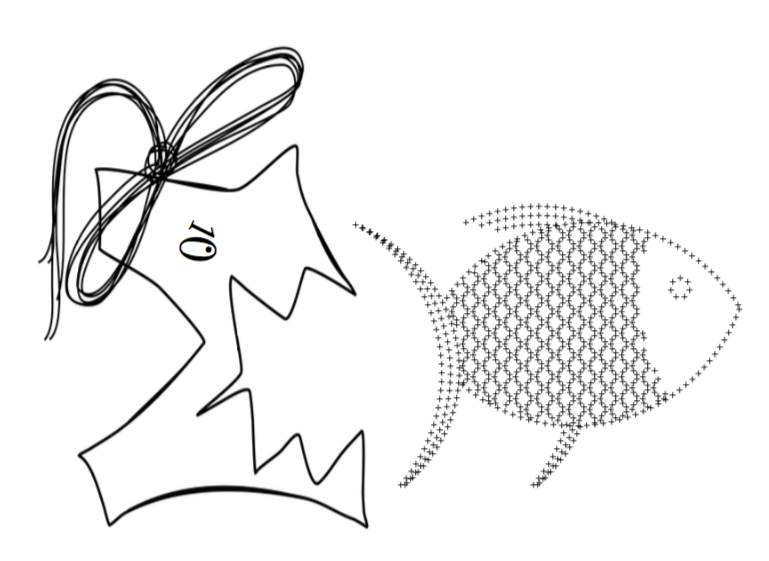
\includegraphics[height=3.2cm,trim={0 0.5cm 0 0.48cm},clip]{outreachlogo.png}

\end{figure}
\end{textblock}

\end{frame}
\end{document}
